% ============================================================
%  INFOGRAPHIC TEMPLATE — Dark background, tcolorbox, TikZ
%  Ispirato allo stile "Kyungu Formula"
%  Compilare con: pdflatex (2 passate)
% ============================================================
%\documentclass[a4paper, 10pt]{article}


% ── Layout ──────────────────────────────────────────────────
%\usepackage[a4paper,
%            top=1.5cm, bottom=1.5cm,
%            left=1.2cm, right=1.2cm]{geometry}

\documentclass[a3paper, 12pt]{article}
\usepackage[a3paper, margin=20mm]{geometry}
\usepackage{multicol}
\setlength{\columnsep}{0.6cm}

% ── Colori e grafica ────────────────────────────────────────
\usepackage[table]{xcolor}
\usepackage{graphicx}
\usepackage{tikz}
\usetikzlibrary{arrows.meta, shapes.geometric, positioning,
                decorations.pathmorphing, backgrounds}
\usepackage{eso-pic}          % sfondo pagina intera

% ── Box colorati ────────────────────────────────────────────
\usepackage[most]{tcolorbox}
\usepackage{mdframed}

% ── Font ────────────────────────────────────────────────────
\usepackage[T1]{fontenc}
\usepackage[utf8]{inputenc}
% microtype removed (not available)

% ── Matematica ──────────────────────────────────────────────
\usepackage{amsmath, amssymb, amsthm}
\usepackage{bm}               % bold math

% ── Icone ───────────────────────────────────────────────────
      % \textbullet, \textbf{!}, ecc.

% ── Varie ───────────────────────────────────────────────────
\usepackage{enumitem}
\usepackage{setspace}
\usepackage{parskip}
\setlength{\parindent}{0pt}
\pagestyle{empty}

% ============================================================
%  PALETTE COLORI  (modifica qui per cambiare tema)
% ============================================================
\definecolor{bgDark}     {HTML}{0D1B2A}   % sfondo pagina
\definecolor{bgMid}      {HTML}{1A2E42}   % box secondari
\definecolor{accentGold} {HTML}{C9A84C}   % oro/giallo titoli
\definecolor{accentBlue} {HTML}{4A9EDB}   % azzurro accenti
\definecolor{accentGreen}{HTML}{4CAF50}   % verde check
\definecolor{accentRed}  {HTML}{E74C3C}   % rosso avvisi
\definecolor{boxOrange}  {HTML}{E8976A}   % box warm
\definecolor{boxPurple}  {HTML}{7B68EE}   % box viola
\definecolor{textLight}  {HTML}{E8EAF0}   % testo chiaro
\definecolor{textMuted}  {HTML}{A0AABB}   % testo secondario

% ============================================================
%  SFONDO PAGINA INTERA
%  Opzione A: colore piatto (attiva di default)
%  Opzione B: immagine — decommentare le 2 righe sotto
% ============================================================
\AddToShipoutPictureBG{%
  \AtPageLowerLeft{%
    \color{bgDark}\rule{\paperwidth}{\paperheight}%
  }%
}
% Opzione B — immagine di sfondo:
% \AddToShipoutPictureBG{\includegraphics[width=\paperwidth,height=\paperheight]{background.jpg}}

% ============================================================
%  STILI tcolorbox
% ============================================================

% Box numerato con header (stile sezione 2.1, 2.2 ...)
\tcbset{
  sectionbox/.style={
    enhanced, breakable,
    colback=bgMid, colframe=accentBlue,
    coltext=textLight,
    arc=4pt, outer arc=4pt,
    boxrule=0.8pt,
    left=6pt, right=6pt, top=5pt, bottom=5pt,
    fonttitle=\bfseries\color{white},
    attach boxed title to top left={yshift=-2mm, xshift=4mm},
    boxed title style={colback=accentBlue, arc=3pt, boxrule=0pt},
  }
}

% Box formula (sfondo caldo)
\tcbset{
  formulabox/.style={
    enhanced,
    colback=boxOrange!15!bgMid, colframe=boxOrange,
    coltext=textLight,
    arc=4pt, boxrule=0.8pt,
    left=8pt, right=8pt, top=6pt, bottom=6pt,
  }
}

% Box nota/definizione (neutro)
\tcbset{
  notebox/.style={
    enhanced,
    colback=bgMid, colframe=textMuted,
    coltext=textLight,
    arc=3pt, boxrule=0.5pt,
    left=6pt, right=6pt, top=4pt, bottom=4pt,
  }
}

% Box highlight gold
\tcbset{
  goldbox/.style={
    enhanced,
    colback=accentGold!20!bgMid, colframe=accentGold,
    coltext=textLight,
    arc=4pt, boxrule=0.8pt,
    left=6pt, right=6pt, top=5pt, bottom=5pt,
    fonttitle=\bfseries\color{accentGold},
    attach boxed title to top left={yshift=-2mm, xshift=4mm},
    boxed title style={colback=accentGold!80!black, arc=3pt, boxrule=0pt},
  }
}

% ============================================================
%  COMANDI UTILITÀ
% ============================================================
\newcommand{\sectionnum}[1]{%
  \tikz[baseline=-0.5ex]\node[fill=accentBlue, text=white,
    font=\bfseries\small, inner sep=3pt, rounded corners=2pt]{#1};%
}

\newcommand{\checkitem}{\textcolor{accentGreen}{\textbullet}\;}
\newcommand{\warnitem}{\textcolor{accentRed}{\textbf{!}}\;}

% Freccia numerata per workflow orizzontale
\newcommand{\workflowstep}[2]{%
  \begin{tcolorbox}[notebox, width=0.28\linewidth,
                    halign=center, valign=center,
                    fontupper=\small]
    \textcolor{accentGold}{\Large\bfseries #1}\\[2pt]
    \textcolor{textLight}{#2}
  \end{tcolorbox}%
}

% ============================================================
%  DOCUMENTO
% ============================================================
\begin{document}

% ── TITOLO ──────────────────────────────────────────────────
\begin{center}
  {\fontsize{28}{32}\selectfont\bfseries\color{accentGold}
    IL TUO TITOLO PRINCIPALE}\\[4pt]
  {\large\color{accentBlue}\bfseries SOTTOTITOLO TECNICO}\\[2pt]
  {\normalsize\color{textMuted}\itshape
    Una formula unificata / breve descrizione}
\end{center}

\vspace{0.3cm}

% ── BANNER INTRO ────────────────────────────────────────────
\begin{tcolorbox}[enhanced, colback=accentBlue!25!bgMid,
                  colframe=accentBlue, coltext=textLight,
                  arc=4pt, boxrule=0.8pt,
                  left=8pt, right=8pt, top=5pt, bottom=5pt]
  \textcolor{accentGold}{\textbf{*}}\quad
  \textbf{Frase introduttiva chiave:} descrizione concisa
  dell'argomento trattato nell'infografica, valida per $ t \ge 0 $.
\end{tcolorbox}

\vspace{0.4cm}

% ── LAYOUT A 2 COLONNE ──────────────────────────────────────
\begin{multicols}{2}

% -------- SEZIONE 2.1 ----------------------------------------
\begin{tcolorbox}[sectionbox,
  title={\sectionnum{2.1}\quad CASO SPECIALE: SERIE INTERA}]

Testo introduttivo della sezione. La formula principale
è mostrata nel box seguente:

\begin{tcolorbox}[formulabox]
\[
  \mathcal{L}^{-1}\bigl[F(p)\bigr](t)
  = \varphi(0)\,\delta(t)
    + \sum_{n=1}^{\infty}
      \frac{\varphi^{(n)}(0)}{(n!)^2}\,n\,t^{n-1}
\]
\end{tcolorbox}

\vspace{4pt}
dove \quad
\begin{tcolorbox}[notebox, width=0.45\linewidth]
$\varphi(x) = F\!\left(\dfrac{1}{x}\right)$
\end{tcolorbox}

\vspace{4pt}
\textcolor{textMuted}{\small
  \(\underbrace{\hspace{1.8cm}}_{\text{termine impulsivo}}\)
  \hspace{0.3cm}
  \(\underbrace{\hspace{2.8cm}}_{\text{contributi regolari, } t>0}\)
}

\end{tcolorbox}

\vspace{0.3cm}

% -------- SEZIONE 2.2 ----------------------------------------
\begin{tcolorbox}[sectionbox,
  title={\sectionnum{2.2}\quad ESTENSIONE GENERALE}]

Sia $F(p)$ definita per $\Re(p)>0$ e si ponga
$\varphi(x)=F(1/x)$ come funzione ausiliaria.

Si assuma che $\varphi(x)$ ammetta, in un intorno di $x=0$,
un'espansione:
\[
  \varphi(x) = \sum_{n=0}^{\infty} c_n\, x^{\alpha_n}, \qquad
  \alpha_n \in \mathbb{R},\quad \alpha_0 \le \alpha_1 \le \cdots
\]

\begin{tcolorbox}[formulabox]
\[
  \mathcal{L}^{-1}[F](t)
  = \underbrace{
      \sum_{\substack{\alpha_n \notin \mathbb{Z}^- \\ \alpha_n \ne 0}}
      \!\!\frac{c_n}{\Gamma(\alpha_n)}\,t^{\alpha_n - 1}
    }_{\text{parte regolare}}
  +\; \underbrace{
      \sum_{\alpha_j = -m} c_j\,\delta^{(m)}(t)
    }_{\text{distribuzioni}}
  +\; \underbrace{
      \sum_{\alpha_k = 0} c_k\,\delta(t)
    }_{\text{impulsivi}}
\]
\end{tcolorbox}

\end{tcolorbox}

\columnbreak   % ← forza il salto di colonna

% -------- BOX NOTAZIONE ─────────────────────────────────────
\begin{tcolorbox}[goldbox, title={NOTAZIONE}]
\renewcommand{\arraystretch}{1.4}
\begin{tabular}{@{}cl@{\quad}l@{}}
  \textcolor{accentGold}{\small$\lambda$} &
    $\delta(t)$       & distribuzione di Dirac \\
  \textcolor{accentGold}{\small$\delta^{(m)}$} &
    $\delta^{(m)}(t)$ & derivata $m$-esima del delta \\
  \textcolor{accentGold}{\small$\Gamma$} &
    $\Gamma(z)$       & funzione Gamma \\
  \textcolor{accentGold}{\small$t_+^\lambda$} &
    $t_+^\lambda$     & distribuzione omogenea \\
\end{tabular}
\end{tcolorbox}

\vspace{0.3cm}

% -------- OSSERVAZIONI ───────────────────────────────────────
\begin{tcolorbox}[notebox, title={\color{accentGold}\bfseries OSSERVAZIONI}]
\begin{itemize}[leftmargin=*, itemsep=2pt]
  \item[\checkitem] Include il caso particolare delle serie intere (Sez.\ 2.1).
  \item[\checkitem] Valida per esponenti reali (non necessariamente interi).
  \item[\checkitem] Unifica contributi regolari, impulsivi e distribuzionali.
\end{itemize}
\end{tcolorbox}

\end{multicols}

\vspace{0.4cm}

% ── WORKFLOW ORIZZONTALE (1→2→3) ────────────────────────────
\begin{tcolorbox}[enhanced, colback=bgMid, colframe=accentBlue,
                  coltext=textLight, arc=4pt,
                  title={\color{white}\bfseries IDEA FONDAMENTALE}]

\begin{center}
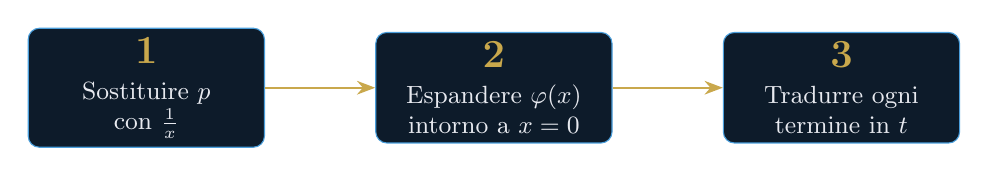
\begin{tikzpicture}[
  node distance = 1.4cm,
  box/.style = {rectangle, rounded corners=4pt,
                fill=bgDark, draw=accentBlue,
                text=textLight, minimum width=3cm,
                minimum height=1.1cm, align=center,
                font=\small},
  arr/.style = {-Stealth, thick, color=accentGold}
]
  \node[box] (n1) {\textcolor{accentGold}{\Large\bfseries 1}\\[2pt]
                    Sostituire $p$\\con $\tfrac{1}{x}$};
  \node[box, right=of n1] (n2)
                  {\textcolor{accentGold}{\Large\bfseries 2}\\[2pt]
                    Espandere $\varphi(x)$\\intorno a $x=0$};
  \node[box, right=of n2] (n3)
                  {\textcolor{accentGold}{\Large\bfseries 3}\\[2pt]
                    Tradurre ogni\\termine in $t$};
  \draw[arr] (n1) -- (n2);
  \draw[arr] (n2) -- (n3);
\end{tikzpicture}
\end{center}

\end{tcolorbox}

\vspace{0.4cm}

% ── ESEMPIO ILLUSTRATIVO ────────────────────────────────────
\begin{tcolorbox}[sectionbox,
  title={\sectionnum{EX}\quad ESEMPIO ILLUSTRATIVO}]

\begin{multicols}{3}

\textbf{\color{accentGold}\textbf{1} Funzione ausiliaria}

Sia $F(p) = \dfrac{1}{p+a}$, con $a>0$.

\[
  \varphi(x) = F\!\left(\tfrac{1}{x}\right)
  = \frac{x}{1+ax}
\]

\columnbreak

\textbf{\color{accentGold}\textbf{2} Espansione intorno a $x=0$}

\[
  \varphi(x) = x(1+ax)^{-1}
  = \sum_{n=1}^{\infty}(-a)^{n-1} x^n
\]
$(c_n = (-a)^{n-1},\; \alpha_n = n \ge 1)$

\columnbreak

\textbf{\color{accentGold}\textbf{3} Risultato}

\[
  \mathcal{L}^{-1}\!\left[\frac{1}{p+a}\right]\!(t)
  = \sum_{n=1}^{\infty}\frac{\varphi^{(n)}(0)}{(n!)^2}\,n\,t^{n-1}
\]

\begin{tcolorbox}[formulabox]
\[
  = e^{-at}, \quad t \ge 0
\]
\end{tcolorbox}

\end{multicols}

\end{tcolorbox}

\vspace{0.4cm}

% ── KEY POINTS (footer) ──────────────────────────────────────
\begin{tcolorbox}[enhanced, colback=bgMid, colframe=accentGold,
                  coltext=textLight, arc=4pt, boxrule=1pt,
                  title={\color{accentGold}\bfseries\large KEY POINTS}]

\begin{multicols}{4}
\begin{center}
  \textcolor{accentGold}{\huge\textbf{O}}\\[4pt]
  \textbf{\color{accentGold}Formula unificata}\\[2pt]
  \small Copre serie intere e non intere.
\end{center}

\columnbreak
\begin{center}
  \textcolor{accentBlue}{\huge\textbf{[S]}}\\[4pt]
  \textbf{\color{accentBlue}Potente in pratica}\\[2pt]
  \small Ideale per funzioni complesse.
\end{center}

\columnbreak
\begin{center}
  \textcolor{accentGreen}{\huge\textbf{!}}\\[4pt]
  \textbf{\color{accentGreen}Senso delle distribuzioni}\\[2pt]
  \small Considera impulsi e derivate del delta.
\end{center}

\columnbreak
\begin{center}
  \textcolor{boxOrange}{\huge\textbf{*}}\\[4pt]
  \textbf{\color{boxOrange}Strumento avanzato}\\[2pt]
  \small Per PDE, teoria della summabilità.
\end{center}

\end{multicols}
\end{tcolorbox}

\end{document}
